\documentclass[12pt]{article}
\usepackage[utf8]{inputenc}
\usepackage{upquote}
\usepackage[margin=1in]{geometry} 
\usepackage{amsmath,amsthm,amssymb}
\usepackage{graphicx}
\usepackage{listings}
\newenvironment{statement}[2][Statement]{\begin{trivlist}
\item[\hskip \labelsep {\bfseries #1}\hskip \labelsep {\bfseries #2.}]}{\end{trivlist}}
\usepackage{xcolor}




\title{Assignment 6}


\author{Author \\
  Wanjing Hu / fng685@alumni.ku.dk  \\
  Zhigao Yan / sxd343@alumni.ku.dk  \\
  Wenshuo Dong / gnj461@alumni.ku.dk  \\
  Jiayi Zhang / xrw579@alumni.ku.dk \\
} 
 

\begin{document}
\maketitle

\section{Question1 $P_1$}
%zhigao
\begin{figure}[h]
    \centering
    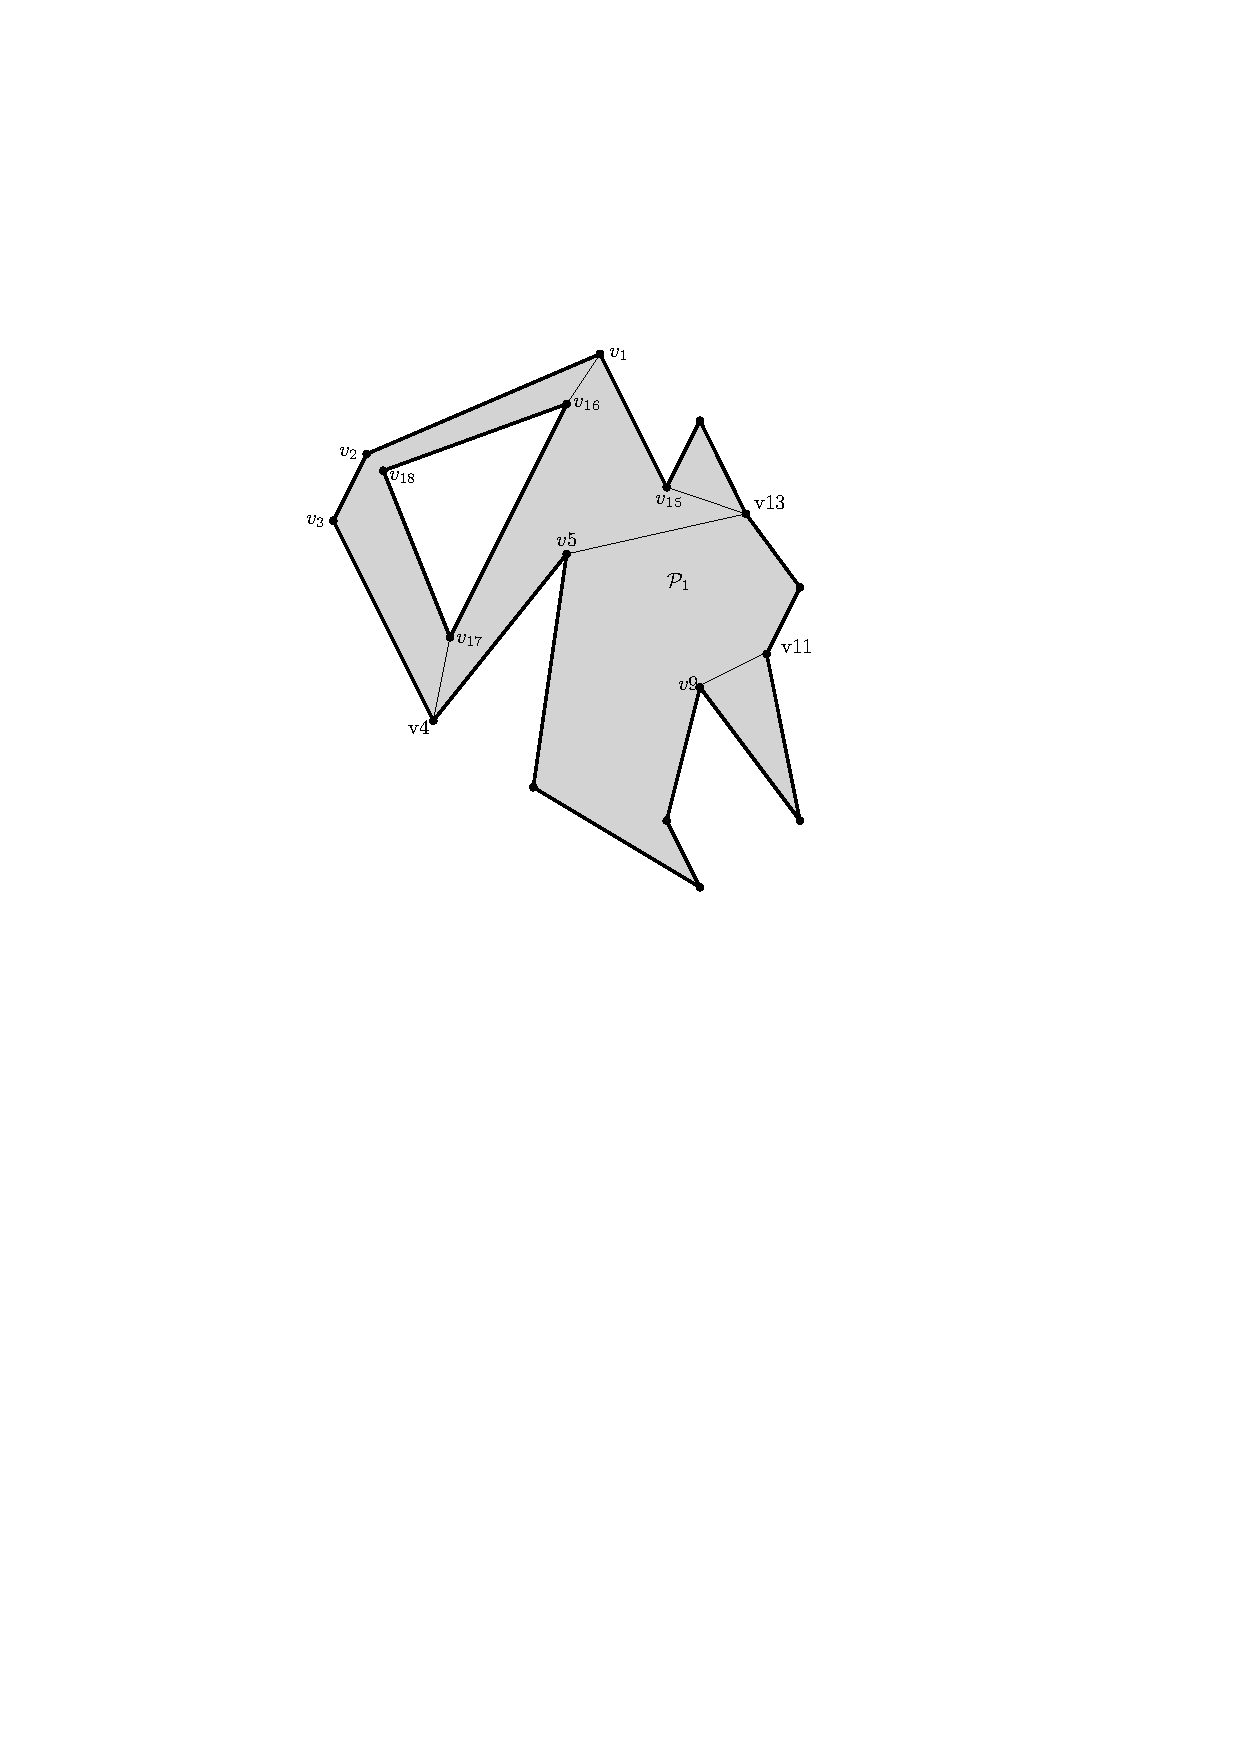
\includegraphics[width=0.5\linewidth]{triangulationExercise (2)-1.pdf}
    \caption{Question 1.a}
    \label{fig:enter-label}
\end{figure}
I use the method from the Computational Geometry book that handles everything in one pass.
The order of the diagonal that I created:

\[v_{16} \rightarrow v_1\]
\[v_{13} \rightarrow v_{15}\]
\[v_{5} \rightarrow v_{13}\]
\[v_{9} \rightarrow v_{11}\]
\[v_{4} \rightarrow v_{17}\]



\section{Question1 $P_2$}
%wenshuo
\begin{figure}[h]
    \centering
    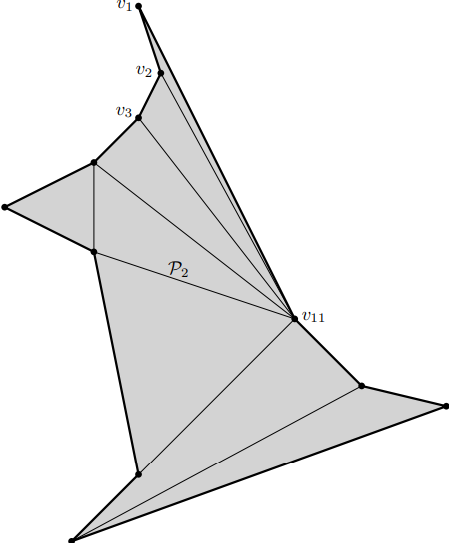
\includegraphics[width=0.5\linewidth]{1b.png}
    \caption{Question 1.b}
    \label{fig:enter-label}
\end{figure}
\[v_{2} \rightarrow v_{11}\]
\[v_{3} \rightarrow v_{11}\]
\[v_{4} \rightarrow v_{11}\]
\[v_{4} \rightarrow v_{6}\]
\[v_{6} \rightarrow v_{11}\]
\[v_{7} \rightarrow v_{11}\]
\[v_{8} \rightarrow v_{10}\]
\section{Exercises 3.4}
%jiayi
\textbf{Question:}
Suppose that a simple polygon P with n vertices is given, together with a set of diagonals that partitions P into convex quadrilaterals. How many cameras are sufficient to guard P? Why doesn’t this contradict the Art Gallery Theorem?\\
\textbf{Answer:} 
From the polygon P can be divided into a set of convex quadrilaterals it follows that n = 2 * t + 4 where $t \geq 0$. This conclusion can easily be deduced by contraposition where we suppose that n =  2 * t + 5.\\
Then we can consider the range of n from 4 to 2*t + 4, every time we add two vertices, it is equal to add a convex quadrilaterals on the base of the last polygon.\\
And the best position of a camera is the diagonals which is a communal edge of two quadrilaterals so it can guard two quadrilaterals.\\
So suppose that the minimum number of cameras is $x$, $x = 1$ when n = 2*0 + 4 or 2*1 + 4, $x = 2$ when we add the third and forth quadrilaterals(where n = 8 or 10), so we can deduce that $x \leq \lceil \frac{t + 1}{2}\rceil = \lceil \frac{n}{4}\rceil \leq \frac{n}{3} $ (where the Art Gallery Theorem given).\\
So $\frac{n}{4}$ cameras are sufficient, and it doesn't contradict the Art Gallery Theorem because the number we calculated is smaller than the upper bound it given.


\section{Exercises 3.7}
%wanjing
There are 2 extra vertices  per diagonal and $\leq n-3$ diagonals, so there are at most  $n+2*(n-3)=3n-6$ vertices.$O(3n-6) = O(n)$


\end{document}
